\section{Login} {
    Per effettuare il login, è possibile eseguirlo accedendo all'applicazione tramite il link riportato sotto e, dopo il redirect automatico, scegliere l'opzione di ``Sign in''. 
    \begin{center}
        \textbf{\url{https://d18v2wlpbu3jpw.cloudfront.net/}}
    \end{center}
    \subsection{Login manuale} {
        L'utente per accedere alla piattaforma deve cliccare il pulsante ``\textbf{Sign in}'', succesivamente verrà indirizzato ad una nuova pagina, 
        la quale contiene il form da compilare. I campi da inserire sono: 
        \begin{itemize}
            \item Username;
            \item Password.
        \end{itemize}
        \begin{figure}[H]
            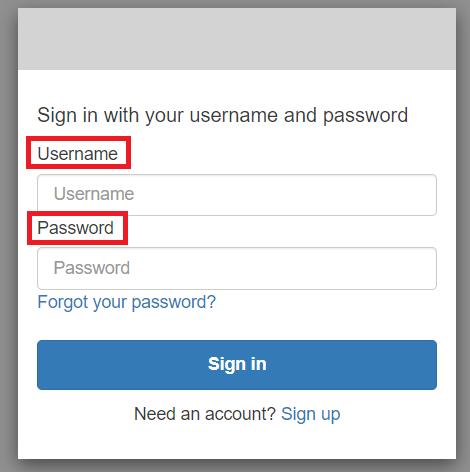
\includegraphics[width=8cm]{sezioni/images/form-log.png}
            \centering
            \caption{Campi di compilazione per il login}
        \end{figure}
        I dati da inserire sono esattamente quelli con cui era avvenuta la registrazione. \aCapo
        Per accedere alla piattoforma è necessario premere il bottone ``\textbf{Sign in}''. 
        \begin{figure}[H]
            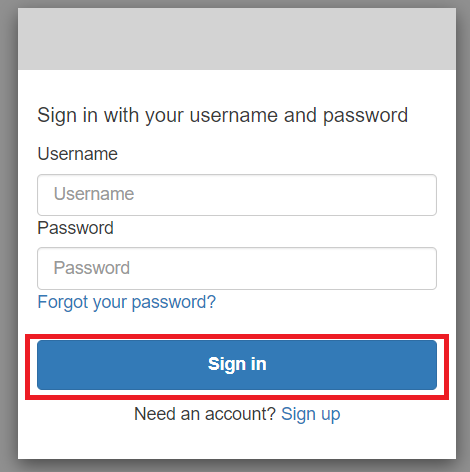
\includegraphics[width=8cm]{sezioni/images/conf-log.png}
            \centering
            \caption{Bottone di conferma per il login}
        \end{figure}
        Se andrà a buon fine, l'utente una volta entrato nella piattaforma potrà visitare la propria home, accedere all'area personale ed infine usufruire dei servizi disponibili da \platform.
    \subsection{Inserimento delle credenziali errate} {
            Se uno o entrambi i campi del modulo di Login non vengono completati, il sistema darà errore come si vede dalla figura. 
            \begin{figure}[H]
                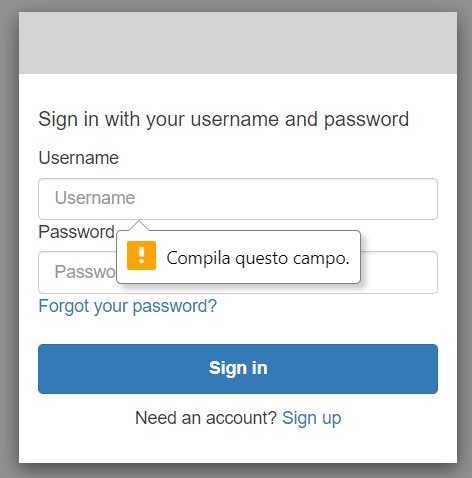
\includegraphics[width=8cm]{sezioni/images/err-vuoto-log.png}
                \centering
                \caption{Segnalazione errore campo vuoto login}
            \end{figure}
            Infatti per accedere è necessario completare i campi, e assicurarsi
            che essi contengano le credenziali scritte corretamente, altrimenti verrà segnalato un errore di quest'altro tipo: 
            \begin{figure}[H]
                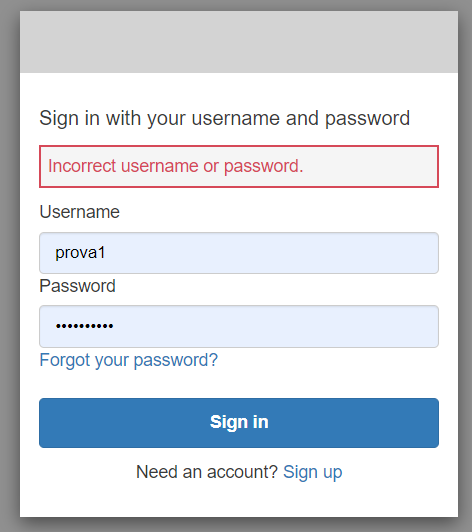
\includegraphics[width=8cm]{sezioni/images/err-log.png}
                \centering
                \caption{Segnalazione errore username o password durante il login}
            \end{figure}
            }   
    }

    \subsection{Login automatico} {
        Se l'utente durante una sessione precedente non ha effettuato il logout, una volta che proverà nuovamente ad accedere alla piattaforma,  
         verrà reindirizzato direttamente alla pagina home, perchè non sarà necessario inserire nuovamente le proprie credenziali. 
         Gli verrà chiesto se vuole accedere con l'account con cui stava navigando nella sessione precedente o se vuole cambiarlo.
         \begin{figure}[H]
            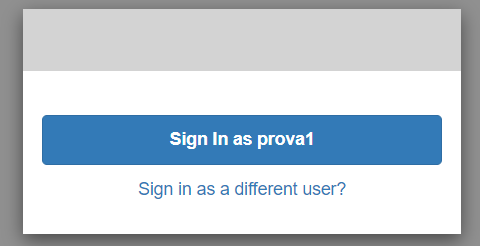
\includegraphics[width=8cm]{sezioni/images/login-auto.png}
            \centering
            \caption{Login automatico}
        \end{figure}
    }
    
    \subsection{Logout} {
        Quando un utente sta navigando all'interno di \platform, per uscire da essa deve eseguire il logout. Per farlo deve cliccare sul bottone ``\textbf{Account}'', il quale lo reindirizzerà ad una nuova pagina,
        nella quale saranno presente le informazioni personali e il bottone ``\textbf{Logout}'' che gli permeterrà di uscire da \platform. 
          
    }




}
